%This is chapter 2
%%=========================================
\chapter{Theoretical basis}

%%=========================================
\section{Agile methods}
\subsection{Scrum}
Scrum is an agile methodology. 
Background and history of the evolution of scrum......
What is it? How does it work?

\subsection{Kanban}

\section{Open source}
Short description of what it is.. Why it is good?
Community engagement... 
\subsection{Licenses}
Do i need this?

\section{Git}
Git is a type of version control system. It was created by .... and is today the most popular VCS.

\subsection{GitFlow}
GitFlow is a popular branching model for Git, created by \cite{gitflow}. Figure \ref{fig:gitflow} displays an example git history, adhering the GitFlow branching style.
\begin{figure}[h]
    \centering
    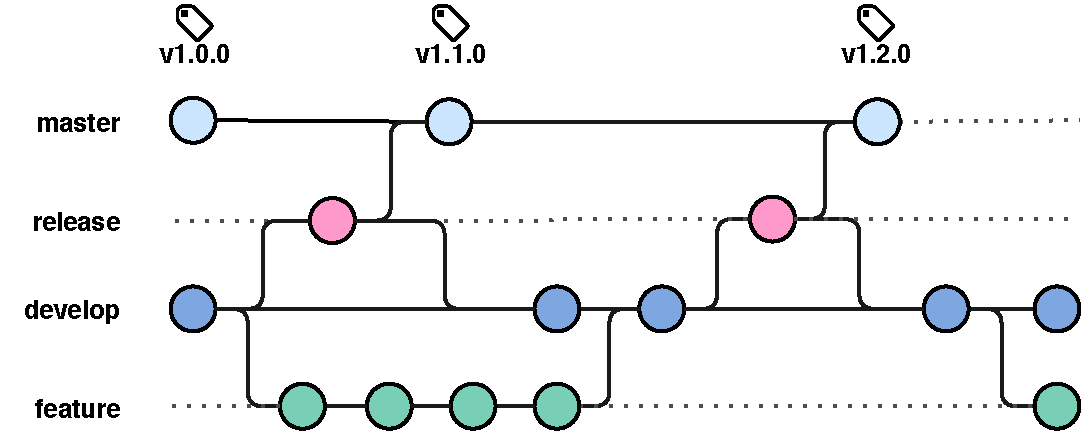
\includegraphics[page=1,width=\textwidth]{sections/methodology/figures/gitflow.pdf}
    \caption{GitFlow branching model example.}
    \label{fig:gitflow}
\end{figure}

\section{GitHub}
GitHub is primarily a hosting service for Git repositories. However, GitHub also provides a lot of other functionality through it's web-based GUI. They also provide automation (CI/CD), named GitHub Actions, Wikis, Access Controls, Task management tools etc...
\subsection{GitHub Actions}
Need to elaborate here as it is a main part of the thesis....

\subsection{GitHub Pages}
Short description....

\section{HyperText Markup Language (HTML)}
Short about HTML5

\section{Cascading Style Sheets (CSS)}
Short about CSS

\section{JavaScript}
JavaScript - actually named ECMAScript....


some history? =>
%https://github.com/myshov/history-of-javascript/tree/master/4_evolution_of_js_modularity
Short about Node.js... more in a later section.. a server side implementation of the JavaScript engine... 
Also mention Electron...

\subsection{Interpreter}
What does it mean that JS is an interpreter? What is it?

\subsection{ECMAScript versions}

\subsection{Module systems}
\subsubsection{ES6 (ES2015)}
\subsubsection{CommonJS}
\subsubsection{Universal Module Definition (UMD)}
\subsubsection{Asynchronous module definition (AMD)}

\subsection{Package managers}
Various Package registries, like NPM and GitHub Package Registry.
\subsubsection{npm}
(I use this one) --> More info
\subsubsection{Bower}
Asd...
\subsection{Transpilation}
Asd...
\subsubsection{Babel}
Asd...
\subsection{Bundling}
JavaScript bundling is an optimization technique to combine separate resource files into one file. This is done in order to reduce the number of HTTP requests required for a page to load. In addition to the performance gain, bundling is also often done in order to develop a JavaScript application in separate files, also called modules. ...... ES6 modules, CommonJS etc...

\subsubsection{Webpack}
% https://hackernoon.com/a-complete-workshop-build-your-es6-code-into-a-library-using-webpack-80295faeb833
Asd...
\subsubsection{Rollup}
Asd...
\subsubsection{Browserify}
Short section?

\section{TypeScript}
TypeScript is a typed superset of JavaScript that compiles to plain JavaScript. It is open source, and primarily developed and maintained by \footcite{microsoft}.

\section{Node.js}
Short about Node.js... a server side implementation of the JavaScript engine... 
\subsection{Node package manager (NPM)}

\section{Electron}
Short about Node.js... a server side implementation of the JavaScript engine... 

\section{React}
\subsection{JavaScript XML (JSX)}

\section{JSDoc}
Markup language for annotating JavaScript source code files.
JSDoc companion documentation generator: JSDoc3 - see git repo....

\section{Data structures}
Plural names ok?

\subsection{Multidimentional arrays}
Reference ndarray by Mikola Lysenko
%https://github.com/scijs/ndarray
Also discuss Strided Arrays ( in JS?).

\subsection{Octrees}

\subsection{Bounding volume hierarchy }
A bounding volume hierarchy, abbreviated BVH, is a type of tree structure.

\section{Computer graphics}
Faces, vertexes.... What is 3D models built up by? (polygons) triangles... color...
texture maps
Rendered by shaders (pipeline)

\subsection{Ray casting}
The raycasting is demonstrated in figure \ref{fig:raycasting-intersections-example}. A ray is directed towards an object. If it intersects a face

\begin{figure}[h]
    \centering
    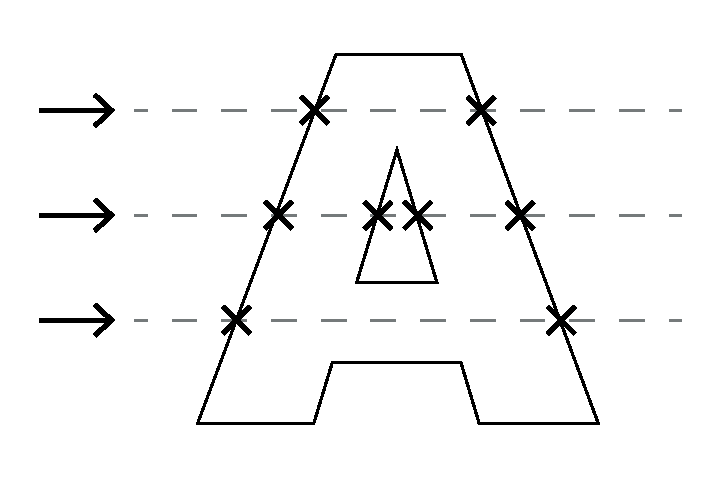
\includegraphics[scale=0.8]{sections/methodology/figures/raycast-intersections}
    \caption{Raycasting intersections example.}
    \label{fig:raycasting-intersections-example}
\end{figure}

\subsection{OpenGL}

\subsection{WebGL}
Uses OpenGl ES, a subset of OpenGL. ...

\subsection{three.js}
three.js abstracts away a lot of the manual handling of constructing vertices, faces, setup of WebGL ....

\section{3D Modeling}
Describe the process and fundamentals of 3D modeling.
UV mapping
Procedural generated texture..
Texture baking
Use Blender etc...
